\documentclass[12pt]{article}

\usepackage{fullpage}
\usepackage{amsmath}
\usepackage{enumerate}
\usepackage{setspace}
\usepackage{bbm}
\usepackage{graphicx}
\usepackage{href}


\title{Econ 828 Term Project:\\ How much is too much?\\
		Beliefs about perceived inequality in a coordination game}
\author{Tim Schulz}
\date{Summer 2016}

\begin{document}
	\maketitle
	\doublespacing
	\section{Introduction}
	\section{Litereature Review}
	\section{Theoretical Framework}
	\subsection{Payoffs}
	The underlying model of the coordination game in this paper is that of a 
	stag hunt with the added dimension of a third party whose decisions 
	potentially affect the payoffs of the other two players who try to 
	coordinate. In the context of inequality, the poor are the parties that 
	play the traditional stag hunt game while the rich person has influence 
	over the exact form of the game by deciding whether to purchase insurance. 
	The resulting payoffs for poor players are shown in Table \ref{gpayoff}.
	
	\begin{table}[!htbp]
		\caption{General Payoffs of Poor}
		\label{gpayoff}
		\begin{center}
		\begin{tabular}{|l|c|c|c|l|c|c|}
			\multicolumn{3}{c}{Under \texttt{no insurance} $(n)$} &
			\multicolumn{1}{c}{} &
			\multicolumn{3}{c}{Under \texttt{insurance} $(i)$}\\
			\cline{1-3}\cline{5-7}
			& revolt & do nothing & & & revolt & do nothing\\
			\cline{1-3}\cline{5-7}
			revolt & $h_n, h_n$ & $l_n, m_n$ && revolt & $h_i, h_i$ & $l_i, 
			m_i$\\
			\cline{1-3}\cline{5-7}
			do nothing & $m_n, l_n$ & $m_n, m_n$ && do nothing & $m_i, l_i$ & 
			$m_i, m_i$\\
			\cline{1-3}\cline{5-7}
		\end{tabular}
		\end{center}
		\footnotesize
		Payoffs of poor players depending on the other poor player's decision 
		and depending on whether the rich person opted for insurance. 
	\end{table}
	
	In order to correctly represent the classical stag hunt game, it has to be 
	the case that the high payoff for successfully coordinating on the payoff 
	dominant strategy is greater than the medium payoff for playing from 
	playing the risk dominant strategy, which in turn is greater than the 
	payoff from unsuccessfully playing the risky strategy. That is, $h_j > m_j 
	> l_j$ in both the \texttt{no insurance} and the \texttt{insurance} case 
	(i.e. $\forall j\in\{n, i\}$). Additionally, successful coordination on the 
	risky action results in the same payoff regardless of the actions of the 
	rich player ($h_n=h_i=h$) and not revolting is risk free not only within a 
	game but also across the two different games resulting from the rich's 
	decisions ($m_n=m_i=m$). Lastly, revolting unsuccessfully is worse if the 
	rich player takes out insurance ($l_i<l_n$) and can be seen as the rich 
	person ``fighting back". These assumptions yield a simplified payoff table 
	for poor players shown in Table \ref{spayoff}.
	
	\begin{table}[!htbp]
		\caption{Simplified Payoffs of Poor}
		\label{spayoff}
		\centering
		\begin{tabular}{|l|c|c|}
			\hline
			& revolt & do nothing\\
			\hline
			revolt & $h, h$ & $l_j, m$\\
			\hline
			do nothing & $m, l_j$ & $m, m$\\
			\hline
		\end{tabular}\\
		\footnotesize Where $j\in\{i, n\}$ and $l_n>l_i$.
	\end{table}
	
	The decision made by the rich player is that of purchasing insurance 
	against a possible revolution. His payoffs depend on whether a revolution 
	was attempted and, if so, whether it was successful. Since a revolutions is 
	only successful if both poor players decide to play the risky action of 
	``revolt" , this case corresponds to the outcome with two revolutionaries. 
	An outcome with only one revolutionary represents an unsuccessful 
	revolution and zero revolutionaries mean nobody tried to revolt.
	
	If a revolutions is successful, having insurance has no effect on the 
	rich's payoffs. That is, in terms of Table \ref{rpayoffs}, 
	$y_{2i}=y{2n}=y_2$. Instead, insurance is only effective in the case of no 
	or failed revolutions (here denoted by the subscript $f$): 
	$y_{0i}=y_{1i}=y{fi}$. This is better than the outcome $y_{1n}$, which 
	represents an attempted but unsuccessful revolutions and can be thought of 
	as being damaging to the rich nonetheless. The best possible outcome for 
	the rich player is not buying insurance and none of the poor attempting a 
	revolution resulting in $y_{0n}$.\footnote{In summary: $y_{0n} > 
	y_{0i}=y_{1i}=y_{fi} > y_{1n} > y_{2i}=y_{2n}=y_2$} Purchasing insurance 
	can therefore be thought of as costing $y_{0n}-y_{fi}$ and paying out 
	$y_{fi}-y_{1n}$ in the case of a failed revolution attempt.
	
	\begin{table}[!htbp]
		\caption{Payoffs of Rich}
		\label{rpayoffs}
		\centering
		\begin{tabular}{|c||c|c|c|c||c|c|}
			\multicolumn{3}{c}{General Form} &
			\multicolumn{1}{c}{} &
			\multicolumn{3}{c}{Simplified Form}\\
			\cline{1-3}\cline{5-7}
			number of & & no & & number of & & no\\
			revolutionaries & insurance & insurance && revolutionaries & 
			insurance & insurance\\
			\cline{1-3}\cline{5-7}
			0 & $y_{0i}$ & $y_{0n}$ && 0 & $y_{fi}$ & $y_{0n}$\\
			\cline{1-3}\cline{5-7}
			1 & $y_{1i}$ & $y_{1n}$ && 1 & $y_{fi}$ & $y_{1n}$\\
			\cline{1-3}\cline{5-7}
			2 & $y_{2i}$ & $y_{2n}$ && 2 & $y_2$ & $y_2$\\
			\cline{1-3}\cline{5-7}
		\end{tabular}
	\end{table}
	
	\subsection{Decision Making Process}
	Given these payoffs, a rational poor player will choose to revolt 
	conditional on beliefs about what the other poor player will do and whether 
	the rich person will buy insurance. Let a poor player believe that the 
	other poor player chooses to revolt with probability $\gamma$ and that the 
	rich player purchases insurance with probability $\delta$. Then a payoff 
	maximizing poor person will revolt if
	$$\gamma h + (1-\gamma)\left[ (1-\delta)l_n + \delta l_i \right] \geq m $$
	
	A rich person will decide to purchase insurance based on his beliefs about 
	how many poor players will choose to revolt. In the most general case, let 
	a rich player believe that there are zero revolutionaries with probability 
	$\alpha$, one revolutionary with probability $\beta$ and two 
	revolutionaries with probability $1-\alpha-\beta$. Then a rich player will 
	purchase insurance if
	\begin{align*}
		(\alpha+\beta)Y_{fi} + (1-\alpha-\beta)y_2 &\geq \alpha y_{0n} + \beta 
		y_{1n} + (1-\alpha-\beta)y_2\\
		(\alpha+\beta)Y_{fi} &\geq \alpha y_{0n} + \beta y_{1n}\\
	\end{align*}
	Assuming independent and identical poor players, $\alpha=(1-\gamma)^2$, 
	$\beta=2\gamma(1-\gamma)$ and $(1-\alpha-\beta)=\gamma^2$. Using this 
	simplification, rich players buy insurance if
	$$ \left[(1-\gamma)^2 + 2\gamma(1-\gamma)\right]y_{fi} \geq 
	(1-\gamma)^2y_{0n} + 2\gamma(1-\gamma)y_{1n} $$
	which simplifies to
	\begin{equation}\tag{I}
		\label{I}
		\gamma \geq \frac{y_{0n} - y_{fi}}{y_{fi} + y_{0n} -2y_{1n}} \equiv 
		\gamma_1.
	\end{equation}
	
	For the decision making process of poor players, this means that if their 
	belief of the other poor player's probability of revolting satisfies 
	condition (\ref{I}), they believe that the rich player will purchase 
	insurance for sure (i.e. $\delta=1$). Considering these second order 
	beliefs, given that $\gamma>\gamma_1$, the poor player chooses to revolt if
	\begin{align*}
		\gamma h + (1-\gamma)l_i &\geq m\\
		\gamma &\geq \frac{m-l_i}{h-l_i} \equiv \gamma_2. \tag{RI}\label{RI}
	\end{align*}
	
	If the poor player believes the other poor player to be sufficiently 
	unlikely to revolt so that the rich player does not purchase insurance 
	(condition (\ref{I}) is not satisfied and $\gamma<\gamma1$), he will only 
	revolt if
	\begin{align*}
		\gamma h + (1-\gamma)l_n &\geq m\\
		\gamma &\geq \frac{m-l_n}{h-l_n} \equiv \gamma_3. \tag{RN}\label{RN}
	\end{align*}
	
	Combining conditions (\ref{I}), (\ref{RI}) and (\ref{RN}), poor players will
	\begin{enumerate}
		\item revolt under insurance if $\gamma \geq \max (\gamma_1, \gamma_2)$
		\item not revolt due to the presence of insurance if $\gamma_1 \leq 
		\gamma < \gamma_2$
		\item revolt under no insurance if $\gamma_3 \leq \gamma < \gamma_1$
		\item not revolt under no insurance if $\gamma < \min (\gamma_1, 
		\gamma_3)$
	\end{enumerate}
	
	\subsection{Possible Ranges of Outcomes}
	Since none of the conditions (\ref{I}), (\ref{RI}) and (\ref{RN}) 
	contradict each other directly, the ranges of $\gamma$ described above can 
	be arranged in various ways by choosing the payoffs of the rich and poor 
	players appropriately. Depending on payoff, some of the cases above can be 
	ruled out from occurring. Possible (rational) outcomes are
	\begin{enumerate}[I.]
		\item 	$0 \leq \gamma_3 < \gamma_1 < \gamma_2 \leq 1$\\
				This is the only arrangement in which all four cases could 
				potentially be observed. With low beliefs about the probability 
				of revolution ($\gamma<\gamma_3$), the rich person does not 
				purchase insurance and poor players do not risk revolting. For 
				a slightly higher perceived probability 
				($\gamma_3\leq\gamma<\gamma_1$), it is still not worth 
				purchasing insurance for the rich player, but poor players 
				still try to revolt. For $\gamma_1\leq\gamma<\gamma_2$, the 
				rich player buys insurance which in turn deters poor players 
				from attempting a revolution as the consequences of failure are 
				now graver than they were without insurance. If a revolution is 
				believed to be likely ($\gamma\geq\gamma_2$), the rich player 
				still purchases insurance on the off-chance that the revolution 
				fails (if the revolution is successful, the outcome for the 
				rich person is the same regardless of insurance) and poor 
				players decide to revolt.
		\item	$0 \leq \gamma_3 < \gamma_2 < \gamma_1 \leq 1$\\
				The rich player does not purchase insurance for values of 
				$\gamma$ below $\gamma_1$. If poor players also believe 
				$\gamma<\gamma_3$, they will not revolt even in the absence of 
				insurance. For $\gamma_3\leq\gamma_1$, poor revolt without 
				facing the rich's insurance. If the beliefs exceed $\gamma_1$, 
				the rich player buys insurance and the poor revolt.
		\item	$0 \leq \gamma_2 < \gamma_3 < \gamma_1 \leq 1$\\
				This case allows for identical outcomes as the one above since 
				$\gamma_2$ is meaningless if $\gamma_2<\gamma_1$.
		\item	$0 \leq \gamma_1 < \gamma_3 < \gamma_2 \leq 1$\\
				There will be no insurance as long as players believe the 
				probability of one poor player to revolt to be less than 
				$\gamma_1$. For values above $\gamma_1$, the rich player buys 
				insurance which deters poor players from revolting as long as 
				beliefs about $\gamma$ are such that $\gamma<\gamma_2$. If the 
				latter condition is not satisfied, the outcome will be a 
				revolution under insurance.
		\item	$0 \leq \gamma_1 < \gamma_2 < \gamma_3 \leq 1$\\
				This is, again, equivalent to the case above as $\gamma_3$ 
				carries no meaning if $\gamma_3 > \gamma_1$.
		\item	$0 \leq \gamma_2 < \gamma_1 < \gamma_3 \leq 1$\\
				This last case only allows for two possible outcomes: No 
				insurance and no revolution if $\gamma<\gamma_1$ or revolution 
				in the presence of insurance if the opposite is believed to be 
				true.
	\end{enumerate}
	
	\section{Experimental Design}
	The experiment follows a $2\times2\time3$ design. First, subjects are 
	randomly assigned either the role of a poor or a rich player. Second, 
	payoffs are designed to have either high or low variation in payoffs for 
	each of the players. Lastly, payoffs are arranged such that the inequality 
	between possible outcomes for poor and rich players is either high, medium 
	or low.
	
	In order to allow for all possible rational action for poor players as 
	discussed in section 3.2, payoffs are chosen such that they meet the 
	requirements of case I. in section 3.3. These payoffs can be seen in Table 
	\ref{allpayoffs}.
	
	\begin{table}[!htbp]
		\caption{Payoff Treatments}
		\label{allpayoffs}
		\centering
		\begin{tabular}{|c|c||c|c|c|c|c|c|c|}
			\multicolumn{2}{c}{Treatment} &\multicolumn{7}{c}{Payoffs}\\
			\hline
			Risk & Inequality & $l_i$ & $l_n$ & $m$ & $h$ & $y_{1n}$ & $y_{fi}$ 
			& $y_{on}$\\
			\hline
			low & low & 130 & 280 & 440 & 750 & 490 & 1100 & 1820\\
			low & medium & 130 & 280 & 440 & 750 & 980 & 2200 & 3640\\
			low & high & 130 & 280 & 440 & 750 & 1960 & 4400 & 7280\\
			high & low & 75 & 130 & 320 & 750 & 500 & 2250 & 4000\\
			high & medium & 75 & 130 & 320 & 750 & 1000 & 4500 & 8000\\
			high & high & 75 & 130 & 320 & 750 & 2000 & 9000 & 16000\\			
			\hline
		\end{tabular}
	\end{table}
	
	Subject are not informed about the existence of these six treatments. 
	Instead, they only know that there are rich and poor players assigned 
	randomly and that two poor players are randomly paired with one rich player 
	into one group.
	
	All players are shown the payoffs selected for the current round. 
	The values from Table \ref{allpayoffs} are filled into Table \ref{spayoff} 
	and into the right side of Table \ref{rpayoffs}. All players see both 
	tables. That way, poor players not only know the risk that they (and the 
	other poor player) face but also how unequal their payoffs are relative to 
	the rich player. Additionally, poor players can see how risky the rich 
	player's possible payoffs are. Based on this information, poor players form 
	beliefs about the the likelihood of the other poor player revolting and the 
	rich player purchasing insurance (which determines which payoff table is 
	relevant for poor players). 
	
	In a similar manner, rich players see their own payoffs and the range 
	between highest and lowest possible outcome on top of how much more they 
	can expect to earn relative to the two poor players in the group and how 
	risky the latter's payoffs are.
	
	Next, poor (rich) players choose whether to revolt (buy insurance). 
	Additionally, rich players are asked to guess whether a revolution will be 
	successful. They are told that guessing correctly is rewarded with 100 
	points.
	Afterwards, all players are informed about how many poor players decided to 
	revolt\footnote{From this, poor players can infer if the other poor player 
	revolted and learn about the likelihood of a revolution based on observed 
	payoffs.} and if insurance was purchased, and all players are told their 
	payoffs from that round.
	
	At the end of a round, each subject is randomly assigned to the role of 
	either a poor or rich player and is furthermore randomly assigned to a new 
	group. Randomizing the order in which subjects play rich or poor players, 
	are faced with high or low risk payoffs, and observe high, medium or low 
	inequality, allows me to ignore any possible order effects.
	
	At the conclusion of the experiment, subjects are paid for three randomly 
	selected periods. Monetary earnings are calculated as $\frac{1}{1000}$ 
	times the points earned in the experiment plus a show-up fee of \$7.
	
	\section{Analysis}
	The focus of this experiment is the subject's belief over the likelihood of 
	successful coordination in response to observed inequality. In the case of 
	poor players, these beliefs are directly observable: A subject should 
	revolt if and only if the other poor player is believed to choose revolt. 
	Therefore, observing a subject's frequency of choosing to revolt, directly 
	represents their belief about the choice of the other poor player. In the 
	case of rich players, this analysis is somewhat less straight-forward. 
	Instead of directly observing the frequency of revolutions, the rich person 
	only indicates whether he believes in a successful revolution. This, 
	however, does not translate directly into $\gamma$ as the probability of 
	both poor players choosing to revolt is $\gamma^2$ as stated previously.
	Assuming that the rich player believes revolutions to be successful with 
	probability $\tau$, the variable of interest is $\sqrt{\tau} = 
	\gamma$. 
	In addition, it is possible to 
	identify a range that the rational rich player must have believed the 
	probability of a revolution to fall in. Using condition (\ref{I}), it is 
	possible to conclude that the rich player must think that $\gamma>\gamma_1$ 
	if he is purchased insurance while the opposite must be true if he did not 
	purchase insurance. This range can be used to verify the validity of using 
	$\sqrt{\tau}$ as the dependent variable in the analysis.
	
	\subsection{Regression Analysis}
	After observing $\gamma$ and $\sqrt{\tau}=\gamma$ for each subject (the 
	former for in cases when subjects were in the role of a poor player and the 
	latter in the role of the rich player) and treatment,\footnote{Assigning 
	the value 1 whenever a poor (rich) person chooses to revolt (buy insurance) 
	and 0 otherwise, the probabilites are the means within a treatment for each 
	subject. This results in six observations per subject.} the goal is to 
	estimate how inequality affects a subject's belief over the probability of 
	a revolution while controlling for risk in the payoffs. The second effect 
	of interest is how perspective changes beliefs or the perception of 
	inequality. This can be quantified as the effect of being assigned either 
	role.

	An appropriate dummy variable model is therefore
	
	\begin{align*}
		\gamma_{it} = b_0 &+ b_1\mathbbm{1}\{inequality_t=medium\}\\
		&+ b_2\mathbbm{1}\{inequality_t=high\}\\
		&+ b_3\mathbbm{1}\{role_t=rich\}\\
		&+ b_4\mathbbm{1}\{risk_t=high\} + \kappa_i + \epsilon_{it}
	\end{align*}
	
	where $b_0$ is the average belief of a poor person playing the game in a 
	low inequality and low risk setup. $b_1$ and $b_2$ identify the effects of 
	of medium and high inequality, respectively. $b_3$ measures how a subject's 
	perspective changes as he switches from the role of a poor player to that 
	of a rich player. The dummy variable whose coefficient is $b_4$ controls 
	for possible risk preferences and $\kappa_i$ captures unobserved 
	heterogeneity among subjects. For example, some subjects might be biased 
	towards thinking that inequality is inherently bad and are therefore more 
	likely to choose to revolt.
	
	Preferably, this model would be estimated using OLS in order to identify 
	linear effects. However, should predicted values of $\gamma_{it}$ fall 
	outside of $[0,1]$, a more appropriate Logit or Probit model would have to 
	be used.
	
	\subsection{Initial Hypothesis}
	A strong positive effect of higher inequality should be observable. Since 
	poor people need to coordinate on one actions, anything from history to 
	social norms suggests that subjects believe that the other subject is more 
	likely to revolt if inequality is greater. Therefore, a reasonable 
	assumption would be that $0<b_1<b_2$.
	
	Next, I would expect rich players to perceive inequality as less pressing 
	than if they observed the same payoff possibilities as a poor person, 
	meaning $b_3<0$. Though theory does not directly predict it, I would also 
	expect $b_3$ to be smaller in magnitude than $b_2$.
	
	Lastly, while the level of risk only serves as a control variable here, a 
	brief discussion of its effect is in order. Risk, as measured in this 
	experiment, only concerns the relative difference between the best and 
	worst possible payoff for a poor player. It is therefore unclear if risk is 
	perceived as the size of a possible loss ($m-l_i$ if insurance is purchased 
	or $m-l_n$ otherwise) or the size of possible gains ($h-m$). The direction 
	of this effect is therefore not clear. The reason risk is a treatment 
	variable in this experiment, is not to measure risk preferences, but rather 
	to control for any possible reaction to risk left after (technically) 
	inducing risk-neutrality by choosing a random round for payment and by 
	doing so to get the least polluted measure of the effect of inequality.
	
	\section{Simulation Exercise}
	A crude implementation in a Monte Carlo simulation\footnote{The script 
	underlying this simulation can be found at \url{}} of the basics of the 
	model presented here verifies the relevance of the proposed research 
	question. The simulation varies from the experiment in a few important 
	aspects. First, ``subjects" (or in this case class instances) do not switch 
	between the roles of poor and rich players. Instead, any initial 
	assignments persist throughout the simulation. Second, the six remaining 
	treatments are not directly implemented. Instead, there is a (near) 
	continuum of treatments. At the beginning of the simulation, 10,000 payoff 
	tables are randomly generated. Of these 10,000, 1,707 satisfied condition 
	the condition that $0 \leq \gamma_3 < \gamma_1 < \gamma_2 \leq 1$, which is 
	necessary to rationally allow for all possible combinations of revolt 
	$\times$ insurance.
	
	Throughout 500 rounds, 30 subjects learned and formed beliefs about the 
	probability of a revolution in response to a variable $d$, which measures, 
	in very simple terms, the degree of inequality and is defined as one minus 
	the ratio of a poor person's payoff relative to that of a rich person if 
	the status quo remained (i.e. nobody revolts and the rich person does not 
	purchase insurance). That is $d=1-\frac{m}{y_{0n}}$. In each round, 
	subjects were randomly assigned into groups of two poor and one rich 
	player. Then, all players were informed about the degree of inequality $d$ 
	in response to which poor players predicted $\gamma$ as a linear function 
	of $d$ and decided to revolt with that probability $\gamma$. Rich players 
	were simulated to purchase insurance if they predicted (based on the Random 
	Forest machine learning algorithm) at least one poor player to revolt. At 
	the end of a round, all simulated players were informed about how many poor 
	players revolted and whether insurance was purchased.
	
	\begin{figure}[!htbp]
		\caption{Simulation Graph}
		\label{simgraph}
		\centering
		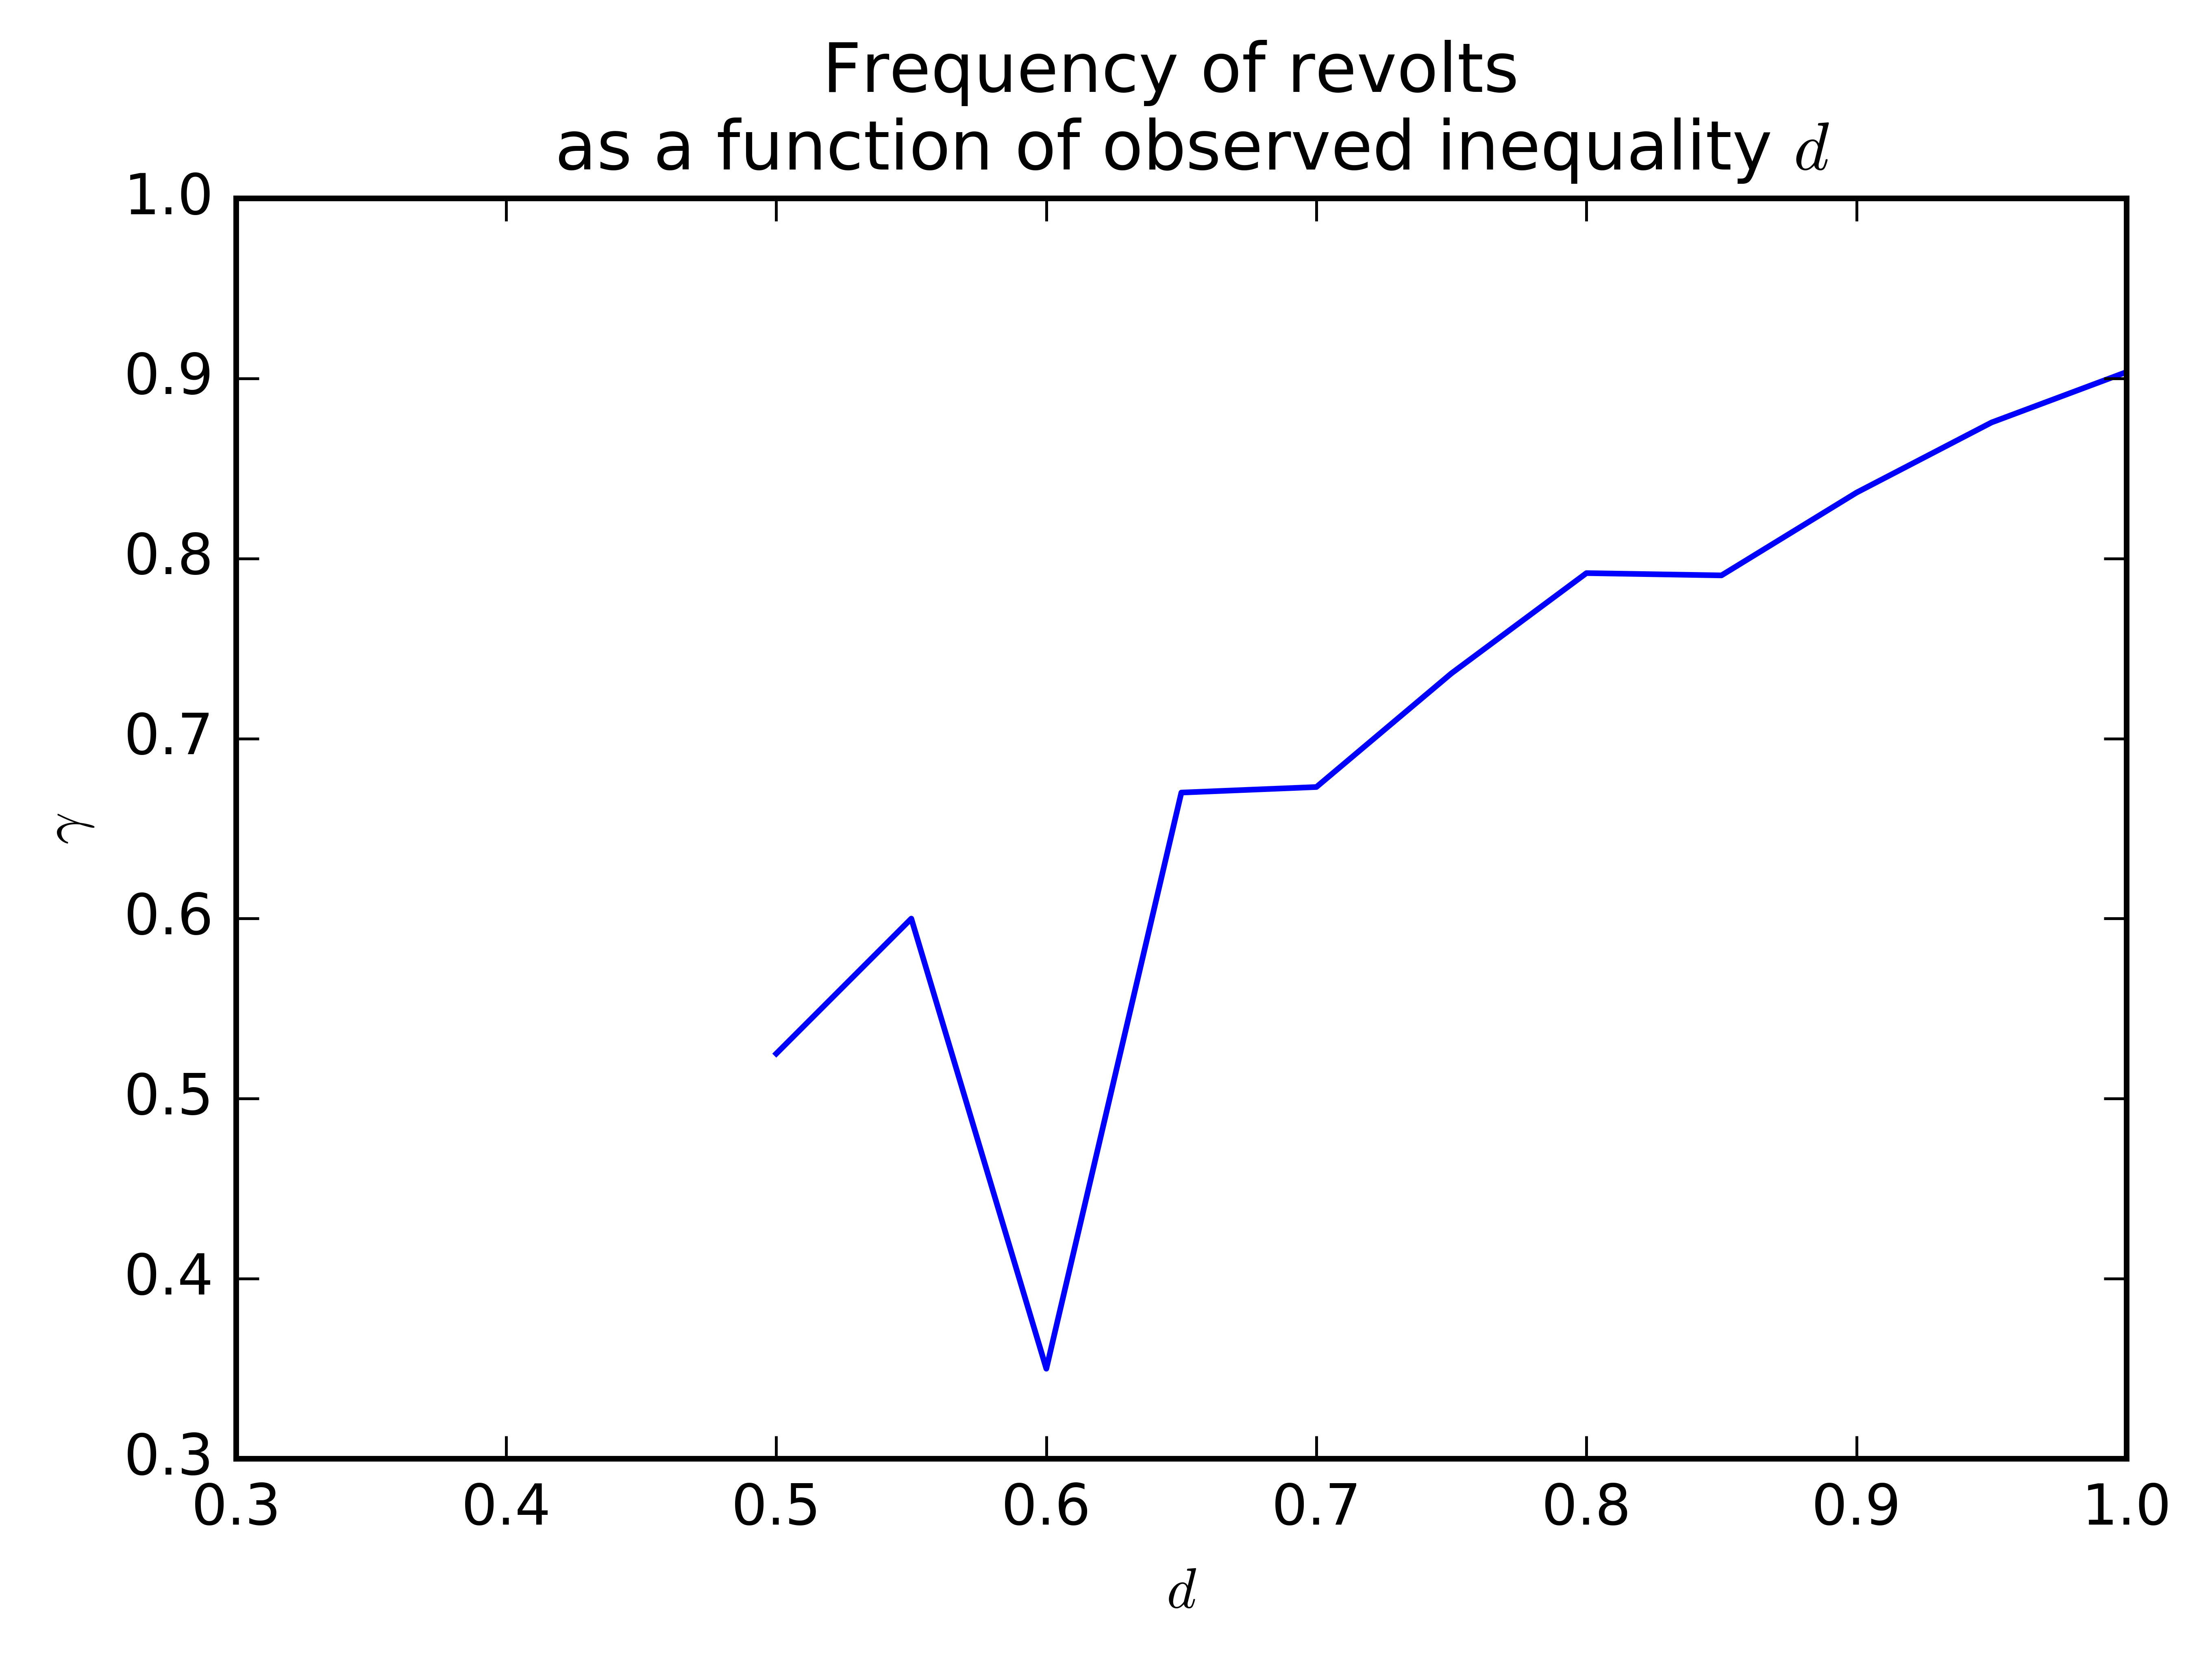
\includegraphics[width=.5\textwidth]{../graph.png}
	\end{figure}
	
	The results of the simulation can be seen in Figure \ref{simgraph}. The 
	graph depicts the observed frequency of poor players choosing to revolt in 
	response to the simplified measure of inequality $d$. As predicted by 
	theory, there is a generally positive relationship between inequality and a 
	poor player's propensity to choose to revolt. The notable exception is the 
	decrease for observations with $d\approx0.6$. This, again, corresponds to 
	theory in the sense that theory predicts a range in which inequality is 
	high enough that rich players purchase insurance, which in turn deters poor 
	players from revolting. Only once inequality keeps increasing, poor players 
	can again coordinate on the risky action of revolting.
	
\end{document}
